%%
%%  AaltoTheses - LaTeX-tutkielmapohjat Aalto-tyylille
%%
%%  Hannu Tiitu
%%  hannu@tiitu.fi
%%
\begin{filecontents*}{\jobname.xmpdata}
  \Title{Evaluation of Managed Kubernetes Solutions for Enterprise Use-cases}
  \Author{Hung Vu}
  \Keywords{cloud native\sep distributed system \sep kubernetes \sep enterprise resource management}
  \Publisher{Aalto University}
\end{filecontents*}
\documentclass[oneside,pdfa,breaklinks]{aaltoseries}
\makeatletter
\@ifpackageloaded{inputenc}{%
  \inputencoding{utf8}}{%
  \usepackage[utf8]{inputenc}}
\hypersetup{hidelinks}              
\makeatother
\usepackage[finnish,english]{babel}   
\usepackage{setspace}                 % Rivivälin säätämiseksi
\usepackage{afterpage}                % Sivun taustaväri
\microtypesetup{letterspace=25}       % Kannen harvaan välistykseen

% My own packages
\usepackage{url}
\def\UrlBreaks{\do\/\do-}
\usepackage{breakurl}
\usepackage{xpatch}
% \usepackage[backend=bibtex,style=ieee,natbib=true]{biblatex}
% \usepackage[style=ieee,backend=biber]{biblatex}
\usepackage[
backend=biber,
sorting=none,
sortcites=true,
defernumbers=false,
bibstyle=ieee,
citestyle=numeric,
]{biblatex}
\AtEveryBibitem{
  \ifentrytype{online}
    {\clearfield{}}
    {\clearfield{url}
     \clearfield{urlyear}
     
    }  % Clear the url and access date fields for non-online entries
}
\xpatchbibdriver{online}
  {\printtext[parens]{\usebibmacro{date}}}
  {\iffieldundef{year}
    {}
    {\printtext[parens]{\usebibmacro{date}}}}
  {}
  {\typeout{There was an error patching biblatex-ieee (specifically, ieee.bbx's @online driver)}}
\addbibresource{references.bib}
\usepackage{xurl}
\usepackage{placeins}


% Bibiography
% \bibliographystyle{IEEEtran}




\author{Hung Vu}
\title{Evaluation of Managed Kubernetes Solutions for Enterprise Use-cases}

\begin{document}



%%  KANSI  ---------------------------------------------

\thispagestyle{empty}
\setcounter{page}{0}  % Kansisivulle sivunumero 0

% Kansisivun marginaalit
\newgeometry{left=23.2mm,right=23.2mm,top=13.5mm,bottom=18mm}

% Punainen kansisivu
\pagecolor{aaltoRed}\afterpage{\nopagecolor}
{\color{black}  % Musta teksti

{\parindent0pt % Kappaleiden sisennys pois päältä
{\fontsize{11.9pt}{11.9pt}\bfseries\sffamily\lsstyle Bachelor’s Programme in Science and Technology}

\color{white}  % Valkoinen teksti alkaa

\vspace{13.1mm}

\begin{spacing}{3.1}
{\fontsize{35}{35}\selectfont Evaluation of Managed Kubernetes Solutions for Enterprise Use-cases}
\end{spacing}

\vspace{2.2mm}

\begin{spacing}{1.24}
{\fontsize{14pt}{14pt}\bfseries\sffamily\lsstyle }
\end{spacing}

\vspace{7.2mm}

\rule{\textwidth}{1.25pt}

\vspace{8.5mm}

{\fontsize{13.9pt}{13.9pt}\bfseries\sffamily\lsstyle Hung Vu}

\vfill

\begin{picture}(0,0)
\put(356,-7.8){\bfseries\sffamily\footnotesize\lsstyle BACHELOR'S}
\put(356,-17.4){\bfseries\sffamily\footnotesize\lsstyle THESIS}
\put(346,-26.5){\rule{.75pt}{25pt}}
\end{picture}

\AaltoLogoSmall{.66}{?}{white}

} % Kappaleiden sisennys takaisin käyttöön
} % Valkoisen tekstin pääätös



%%  NIMIÖSIVU  -----------------------------------------

\newpage

\pagenumbering{roman}

% Nimiösivun marginaalit
\newgeometry{left=80.7mm,right=25mm,top=12.9mm,bottom=21mm}

\thispagestyle{empty}

{\parindent0pt % Kappaleiden sisennys pois päältä
\begin{spacing}{1.1}
\hspace{-39.1mm}{\fontsize{10.5pt}{10.5pt}\sffamily\lsstyle Aalto University}

\hspace{-39.1mm}{\fontsize{10.5pt}{10.5pt}\bfseries\sffamily\lsstyle BACHELOR'S THESIS} {\sffamily\lsstyle 2024}
\end{spacing}

\vspace{12.7mm}

\begin{spacing}{1.63}
{\fontsize{17.8pt}{17.8pt}\selectfont Evaluation of Managed Kubernetes Solutions for Enterprise Use-cases}
\end{spacing}

\vspace{10.5mm}

\begin{spacing}{1.2}
{\fontsize{13pt}{13pt}\selectfont }
\end{spacing}

\vspace{10.6mm}

{\fontsize{13.9pt}{13.9pt}\bfseries\sffamily\lsstyle Hung Vu}

\vfill

{\fontsize{10.3pt}{10.3pt}\sffamily\lsstyle\raggedright
\begin{spacing}{1.06}

Thesis submitted in partial fulfilment of the requirements for the
degree of Bachelor of Science in Technology.

Otaniemi, 25 November 2024

\begin{tabbing}
Supervisor:\hspace{6mm} \= Prof. Gopika Premsankar (Aalto University) \\
Advisor: \> Mr. Daniel Tyrode (Nokia Oy)
\end{tabbing}
\vspace{-4mm}
\end{spacing}
} % fontsize

\vspace{11.5mm}

\begin{spacing}{.9}
{\bfseries\sffamily\lsstyle Aalto University \\
School of Science \\
Bachelor’s Programme in Science and Technology}
\end{spacing}
} % Kappaleiden sisennys takaisin käyttöön



%%  ABSTRACT  ------------------------------------------

\newpage
\phantomsection
\addcontentsline{toc}{chapter}{Abstract}

% Tiivistelmien marginaalit
\newgeometry{left=41.8mm,right=25mm,top=14.33mm,bottom=27mm}
% Alkuperäisessä Aalto-sarjassa marginaalit ovat suunnilleen näin:
%\newgeometry{left=41.8mm,right=17.6mm,top=14.33mm,bottom=20.4mm}

\begin{spacing}{.88}

{\parindent0pt % Kappaleiden sisennys pois päältä
\AaltoLogoSmall{.625}{''}{aaltoBlack}

{\fontsize{13.9pt}{13.9pt}\selectfont
\vspace{-8.9mm}\hfill{\bfseries\sffamily\lsstyle Abstract}}

{\fontsize{9.48pt}{9.48pt}\selectfont
\vspace{.9mm}\hfill{\bfseries\sffamily\lsstyle Aalto University, P.O. Box 11000, FI-00076 Aalto~~\textcolor{aaltoGray}{www.aalto.fi}}}

\vspace{7.8mm}{\fontsize{10.5pt}{10.5pt}\bfseries\sffamily\lsstyle Author}\\
{\small Hung Vu}

\vspace{-2.4mm}\rule{\textwidth}{.75pt}

{\fontsize{10.5pt}{10.5pt}\bfseries\sffamily\lsstyle Title}\\
\parbox[t]{\textwidth}{\raggedright\small Evaluation of Managed Kubernetes Solutions for Enterprise Use-cases}

\vspace{.5mm}\rule{\textwidth}{.75pt}

{\fontsize{10.5pt}{10.5pt}\bfseries\sffamily\lsstyle School}~~{\small School of Science}

\vspace{-2.4mm}\rule{\textwidth}{.75pt}

{\fontsize{10.5pt}{10.5pt}\bfseries\sffamily\lsstyle Degree programme}~~{\small Bachelor’s Programme in Science and Technology}

\vspace{-2.4mm}\rule{\textwidth}{.75pt}

{\fontsize{10.5pt}{10.5pt}\bfseries\sffamily\lsstyle Major}~~{\small Digital Systems and Design}\hfill{\fontsize{10.5pt}{10.5pt}\bfseries\sffamily\lsstyle Code}~~{\small (unknown)}

\vspace{-2.4mm}\rule{\textwidth}{.75pt}

{\fontsize{10.5pt}{10.5pt}\bfseries\sffamily\lsstyle Supervisor}~~{\small Prof. Gopika Premsankar (Aalto University)}

\vspace{-2.4mm}\rule{\textwidth}{.75pt}

{\fontsize{10.5pt}{10.5pt}\bfseries\sffamily\lsstyle Advisor}~~{\small Mr. Daniel Tyrode (Nokia Oy)}

\vspace{-2.4mm}\rule{\textwidth}{.75pt}

{\fontsize{10.5pt}{10.5pt}\bfseries\sffamily\lsstyle Level}~~{\small Bachelor's thesis}\hfill{\fontsize{10.5pt}{10.5pt}\bfseries\sffamily\lsstyle Date}~~{\small 31 May 2024}\hfill{\fontsize{10.5pt}{10.5pt}\bfseries\sffamily\lsstyle Pages}~~{\small 70}\hfill{\fontsize{10.5pt}{10.5pt}\bfseries\sffamily\lsstyle Language}~~{\small English}

\vspace{-2.4mm}\rule{\textwidth}{.75pt}

\vspace{6mm}

} % Kappaleiden sisennys takaisin käyttöön
\end{spacing}
\begin{spacing}{1.05}

\noindent{\fontsize{10.5pt}{10.5pt}\bfseries\sffamily\lsstyle Abstract}
\vspace{.8mm}

{\small
  Abstract here (not required in the research plan)
}

\vfill

\end{spacing}
\begin{spacing}{.88}
{\parindent0pt % Kappaleiden sisennys pois päältä

\makebox[19mm][l]{\fontsize{10.5pt}{10.5pt}\bfseries\sffamily\lsstyle Keywords}\parbox[t]{123.6mm}{\raggedright\small cloud native, distributed systems, kubernetes, enterprise resource management}

\vspace{.5mm}\rule{\textwidth}{.75pt}

{\fontsize{10.5pt}{10.5pt}\bfseries\sffamily\lsstyle urn}~~{\small https://aaltodoc.aalto.fi}

\vspace{-2.4mm}\rule{\textwidth}{.75pt}

} % Kappaleiden sisennys takaisin käyttöön
\end{spacing}



%%  TIIVISTELMÄ  ---------------------------------------

% \newpage
% \phantomsection
% \addcontentsline{toc}{chapter}{Tiivistelmä}

% % Tiivistelmäsivu suomeksi
% \selectlanguage{finnish}

% \begin{spacing}{.88}

% {\parindent0pt % Kappaleiden sisennys pois päältä
% \AaltoLogoSmall{.625}{!}{aaltoBlack}

% {\fontsize{13.9pt}{13.9pt}\selectfont
% \vspace{-8.9mm}\hfill{\bfseries\sffamily\lsstyle Tiivistelmä}}

% {\fontsize{9.48pt}{9.48pt}\selectfont
% \vspace{.9mm}\hfill{\bfseries\sffamily\lsstyle Aalto-yliopisto, PL 11000, 00076 Aalto~~\textcolor{aaltoGray}{www.aalto.fi}}}

% \vspace{7.8mm}{\fontsize{10.5pt}{10.5pt}\bfseries\sffamily\lsstyle Tekijä}\\
% {\small Hung Vu}

% \vspace{-2.4mm}\rule{\textwidth}{.75pt}

% {\fontsize{10.5pt}{10.5pt}\bfseries\sffamily\lsstyle Työn nimi}\\
% \parbox[t]{\textwidth}{\raggedright\small Oikeisiin virheisiin! Virheelliset vastaukset ja niiden tulkinta automaattisesti tarkastetuissa matematiikan harjoitustehtävissä}

% \vspace{.5mm}\rule{\textwidth}{.75pt}

% {\fontsize{10.5pt}{10.5pt}\bfseries\sffamily\lsstyle Korkeakoulu}~~{\small Perustieteiden korkeakoulu}

% \vspace{-2.4mm}\rule{\textwidth}{.75pt}

% {\fontsize{10.5pt}{10.5pt}\bfseries\sffamily\lsstyle Koulutusohjelma}~~{\small Teknistieteellinen kandidaattiohjelma}

% \vspace{-2.4mm}\rule{\textwidth}{.75pt}

% {\fontsize{10.5pt}{10.5pt}\bfseries\sffamily\lsstyle Pääaine}~~{\small Mediatekniikka}\hfill{\fontsize{10.5pt}{10.5pt}\bfseries\sffamily\lsstyle Koodi}~~{\small IL3011}

% \vspace{-2.4mm}\rule{\textwidth}{.75pt}

% {\fontsize{10.5pt}{10.5pt}\bfseries\sffamily\lsstyle Vastuuopettaja}~~{\small professori Lauri Malmi}

% \vspace{-2.4mm}\rule{\textwidth}{.75pt}

% {\fontsize{10.5pt}{10.5pt}\bfseries\sffamily\lsstyle Ohjaaja}~~{\small dosentti Jarmo Malinen}

% \vspace{-2.4mm}\rule{\textwidth}{.75pt}

% {\fontsize{10.5pt}{10.5pt}\bfseries\sffamily\lsstyle Työn laji}~~{\small Kandidaatintyö}\hfill{\fontsize{10.5pt}{10.5pt}\bfseries\sffamily\lsstyle Päiväys}~~{\small 27.11.2017}\hfill{\fontsize{10.5pt}{10.5pt}\bfseries\sffamily\lsstyle Sivuja}~~{\small 70}\hfill{\fontsize{10.5pt}{10.5pt}\bfseries\sffamily\lsstyle Kieli}~~{\small englanti}

% \vspace{-2.4mm}\rule{\textwidth}{.75pt}

% \vspace{6mm}

% } % Kappaleiden sisennys takaisin käyttöön
% \end{spacing}
% \begin{spacing}{1.05}

% \noindent{\fontsize{10.5pt}{10.5pt}\bfseries\sffamily\lsstyle Tiivistelmä}
% \vspace{.8mm}

% {\small
%   Lorem ipsum dolor sit amet, consectetuer adipiscing elit. Ut purus
%   elit, vestibulum ut, placerat ac, adipiscing vitae, felis. Curabitur
%   dictum gravida mauris. Nam arcu libero, nonummy eget, consectetuer
%   id, vulputate a, magna. Donec vehicula augue eu neque. Pellentesque
%   habitant morbi tristique senectus et netus et malesuada fames ac
%   turpis egestas. Mauris ut leo. Cras viverra metus rhoncus sem. Nulla
%   et lectus vestibulum urna fringilla ultrices. Phasellus eu tellus
%   sit amet tortor gravida placerat. Integer sapien est, iaculis in,
%   pretium quis, viverra ac, nunc. Praesent eget sem vel leo ultrices
%   bibendum. Aenean faucibus. Morbi dolor nulla, malesuada eu, pulvinar
%   at, mollis ac, nulla. Curabitur auctor semper nulla.  Donec varius
%   orci eget risus. Duis nibh mi, congue eu, accumsan eleifend,
%   sagittis quis, diam. Duis eget orci sit amet orci dignissim rutrum.

%   Nam dui ligula, fringilla a, euismod sodales, sollicitudin vel,
%   wisi. Morbi auctor lorem non justo. Nam lacus libero, pretium at,
%   lobortis vitae, ultricies et, tellus. Donec aliquet, tortor sed
%   accumsan bibendum, erat ligula aliquet magna, vitae ornare odio
%   metus a mi. Morbi ac orci et nisl hendrerit mollis. Suspendisse ut
%   massa. Cras nec ante. Pellentesque a nulla.  Cum sociis natoque
%   penatibus et magnis dis parturient montes, nascetur ridiculus
%   mus. Aliquam tincidunt urna. Nulla ullamcorper vestibulum
%   turpis. Pellentesque cursus luctus mauris.

%   Nulla malesuada porttitor diam. Donec felis erat, congue non,
%   volutpat at, tincidunt tristique, libero. Vivamus viverra fermentum
%   felis. Donec nonummy pellentesque ante. Phasellus adipiscing semper
%   elit. Proin fermentum massa ac quam. Sed diam turpis, molestie
%   vitae, placerat a, molestie nec, leo. Maecenas lacinia. Nam ipsum
%   ligula, eleifend at, accumsan nec, suscipit a, ipsum. Morbi blandit
%   ligula feugiat magna. Nunc eleifend consequat lorem. Sed lacinia
%   nulla vitae enim. Pellentesque tincidunt purus vel magna. Integer
%   non enim. Praesent euismod nunc eu purus.  Donec bibendum quam in
%   tellus. Nullam cursus pulvinar lectus. Donec et mi. Nam vulputate
%   metus eu enim. Vestibulum pellentesque felis eu massa.
% }

% \vfill

% \end{spacing}
% \begin{spacing}{.88}
% {\parindent0pt % Kappaleiden sisennys pois päältä

% \makebox[21mm][l]{\fontsize{10.5pt}{10.5pt}\bfseries\sffamily\lsstyle Avainsanat}\parbox[t]{121.6mm}{\raggedright\small oppimisympäristö, pedagoginen käytettävyys, virheluokittelu, automaattinen tarkastaminen, matematiikan opetus, Stack}

% \vspace{.5mm}\rule{\textwidth}{.75pt}

% {\fontsize{10.5pt}{10.5pt}\bfseries\sffamily\lsstyle urn}~~{\small https://aaltodoc.aalto.fi}

% \vspace{-2.4mm}\rule{\textwidth}{.75pt}

% } % Kappaleiden sisennys takaisin käyttöön
% \end{spacing}

% \selectlanguage{english}  % Palataan englantiin
% \restoregeometry  % Palataan normaaleihin sivumarginaaleihin



%%  SISÄLTÖ  -------------------------------------------

\newpage

\tableofcontents

%%  TYÖ ALKAA TÄSTÄ  -----------------------------------

\newpage

\pagenumbering{arabic}

\chapter{Introduction}

The cloud is a concept that was first introduced in 2006 with the launch of the first public cloud service (Simple Storage Service, S3 on the 13th of March 2006) \cite{liuReviewDigitalTwin2021}. Since then, the field has experienced rapid growth and development, with the rise of various tools, frameworks, and paradigms. Notably, a core technology that characterises modern cloud computing is \textit{containerisation} \cite{pereiraferreiraPerformanceEvaluationContainers2019}. Through containerisation, application dependencies can be packaged in “containers” that share access to the underlying host OS kernel, allowing multiple containers with different dependencies to be hosted on the same hardware.

While being resource-efficient, the adoption of containers in the cloud faces a new set of challenges in terms of automation, scalability, and management \cite{pereiraferreiraPerformanceEvaluationContainers2019}. To address these challenges, a range of container orchestration tools were developed. The most notable being Kubernetes, an open-source container orchestration platform that was originally developed by Google \cite{Kubernetes, pereiraferreiraPerformanceEvaluationContainers2019}. Although other tools such as Docker Swarm exist, Kubernetes remains as the industry’s de facto standard in terms of container management due to its robust reliability, extensive feature set, and broad ecosystem \cite{truyenComprehensiveFeatureComparison2019}.

Kubernetes can manage hundreds of thousands of containers, making it extremely scalable. In addition to the upstream Kubernetes, various Kubernetes distributions were developed to cater towards specific use-cases, such as edge computing and enterprise environments. In managed Kubernetes for enterprise use-cases in particular, the focus is on providing features like streamlined application deployment, enhanced security, advanced management capability, and optimised resource utilisation for large-scale applications \cite{WhatEnterpriseKubernetes, truyenComprehensiveFeatureComparison2019, jiangIndustrialApplicationsDigital2021}. This combination of scalability and enhanced functionality makes managed Kubernetes a preferred choice for organisations over native Kubernetes and other open-source alternatives \cite{redhatinc.StateKubernetesSecurity2024, vrabicDigitalTwinsUnderstanding2018, portworxKubernetesAdoptionSurvey2021, broadcomStateKubernetes20232023}.

With the ever-growing demand for managed Kubernetes distribution at the enterprise level, multiple service providers such as Amazon, Microsoft, Google, Red Hat, and VMware, all offer their own flavour of Kubernetes (EKS, GKE, AKS, OpenShift, and VMware Tanzu respectively) \cite{AmazonEKSCustomers, maEurekaHumanLevelReward2023, nickomangAzureKubernetesService, redhatinc.RedHatOpenShift, VMwareTanzuPlatform}. Each distribution has its pros and cons, but they all offer a high degree of feature availability that elevates Kubernetes beyond its upstream version with tools for monitoring, scaling, managing, and securing enterprise workloads.

In addition to their varying feature sets, these distributions also differ in terms of their cost structure, which can be further broken down into infrastructure, management, and additional service costs. 

Although Kubernetes distributions' performance are relatively well-researched, few studies look at the managed Kubernetes distributions in terms of features and cost of operation \cite{bohmProfilingLightweightContainer2021, kjorveziroskiKubernetesDistributionsEdge2022, ascensaoAssessingKubernetesDistributions2024, pereiraferreiraPerformanceEvaluationContainers2019}. These aspects, especially the cost, are crucial for companies and organisations to make informed decision on their distribution of choice.

Therefore, this thesis aims to identify the current state of Kubernetes adoption and key challenges to derive key feature requirements for Kubernetes distributions. Based on these requirements, it then compares various distributions and evaluates their ability to address said requirements, as well as the expected cost of operation for each distribution. The goal of this work is to provide a comprehensive assessment of available managed Kubernetes offerings and identify the best-suited options for the industry to meet the most common set of requirements.

Among managed Kubernetes distributions, EKS, GKE, AKS, and OpenShift consistently rank among the most widely adopted distributions for organisations \cite{redhatinc.StateKubernetesSecurity2024, vrabicDigitalTwinsUnderstanding2018, portworxKubernetesAdoptionSurvey2021, broadcomStateKubernetes20232023}. Thus, these four distributions are chosen for assessment to make the work relevant to Nokia and the industry at large. The evaluation consists of three main parts: a brief literature review on the current state of managed Kubernetes distributions, a feature comparison, and a cost analysis for the selected distributions.

The subsequent sections of this thesis are arranged as follows. Section 2 provides background on the relevant technologies to Kubernetes and the mentioned managed Kubernetes distributions. Section 3 outlines the research methodology. Section 4 compiles and interprets results from the review. Lastly, Section 5 concludes the findings and discusses potential topics for further research.

% \section{Fusce mauris}

% Fusce mauris. Vestibulum luctus nibh at lectus. Sed bibendum, nulla a
% faucibus semper, leo velit ultricies tellus, ac venenatis arcu wisi
% vel nisl.  Vestibulum diam. Aliquam pellentesque, augue quis sagittis
% posuere, turpis lacus congue quam, in hendrerit risus eros eget
% felis. Maecenas eget erat in sapien mattis porttitor. Vestibulum
% porttitor. Nulla facilisi.  Sed a turpis eu lacus commodo
% facilisis. Morbi fringilla, wisi in dignissim interdum, justo lectus
% sagittis dui, et vehicula libero dui cursus dui. Mauris tempor ligula
% sed lacus. Duis cursus enim ut augue. Cras ac magna.  Cras
% nulla. Nulla egestas. Curabitur a leo. Quisque egestas wisi eget
% nunc. Nam feugiat lacus vel est. Curabitur consectetuer.

% Suspendisse vel felis. Ut lorem lorem, interdum eu, tincidunt sit
% amet, laoreet vitae, arcu. Aenean faucibus pede eu ante. Praesent enim
% elit, rutrum at, molestie non, nonummy vel, nisl. Ut lectus eros,
% malesuada sit amet, fermentum eu, sodales cursus, magna. Donec eu
% purus. Quisque vehicula, urna sed ultricies auctor, pede lorem egestas
% dui, et convallis elit erat sed nulla. Donec luctus. Curabitur et
% nunc. Aliquam dolor odio, commodo pretium, ultricies non, pharetra in,
% velit. Integer arcu est, nonummy in, fermentum faucibus, egestas vel,
% odio.

% \subsection{Sed commodo posuere pede}

% Sed commodo posuere pede. Mauris ut est. Ut quis purus. Sed ac odio.
% Sed vehicula hendrerit sem. Duis non odio. Morbi ut dui. Sed accumsan
% risus eget odio. In hac habitasse platea dictumst. Pellentesque non
% elit.  Fusce sed justo eu urna porta tincidunt. Mauris felis odio,
% sollicitudin sed, volutpat a, ornare ac, erat. Morbi quis dolor. Donec
% pellentesque, erat ac sagittis semper, nunc dui lobortis purus, quis
% congue purus metus ultricies tellus. Proin et quam. Class aptent
% taciti sociosqu ad litora torquent per conubia nostra, per inceptos
% hymenaeos. Praesent sapien turpis, fermentum vel, eleifend faucibus,
% vehicula eu, lacus.

% Pellentesque habitant morbi tristique senectus et netus et malesuada
% fames ac turpis egestas. Donec odio elit, dictum in, hendrerit sit
% amet, egestas sed, leo. Praesent feugiat sapien aliquet odio. Integer
% vitae justo.  Aliquam vestibulum fringilla lorem. Sed neque lectus,
% consectetuer at, consectetuer sed, eleifend ac, lectus. Nulla
% facilisi. Pellentesque eget lectus. Proin eu metus. Sed porttitor. In
% hac habitasse platea dictumst. Suspendisse eu lectus. Ut mi mi,
% lacinia sit amet, placerat et, mollis vitae, dui. Sed ante tellus,
% tristique ut, iaculis eu, malesuada ac, dui. Mauris nibh leo,
% facilisis non, adipiscing quis, ultrices a, dui.

% \subsection{Morbi luctus}

% Morbi luctus, wisi viverra faucibus pretium, nibh est placerat odio,
% nec commodo wisi enim eget quam. Quisque libero justo, consectetuer a,
% feugiat vitae, porttitor eu, libero. Suspendisse sed mauris vitae elit
% sollicitudin malesuada. Maecenas ultricies eros sit amet ante. Ut
% venenatis velit. Maecenas sed mi eget dui varius euismod. Phasellus
% aliquet volutpat odio. Vestibulum ante ipsum primis in faucibus orci
% luctus et ultrices posuere cubilia Curae; Pellentesque sit amet pede
% ac sem eleifend consectetuer. Nullam elementum, urna vel imperdiet
% sodales, elit ipsum pharetra ligula, ac pretium ante justo a
% nulla. Curabitur tristique arcu eu metus. Vestibulum lectus. Proin
% mauris. Proin eu nunc eu urna hendrerit faucibus. Aliquam auctor, pede
% consequat laoreet varius, eros tellus scelerisque quam, pellentesque
% hendrerit ipsum dolor sed augue. Nulla nec lacus.

% Suspendisse vitae elit. Aliquam arcu neque, ornare in, ullamcorper
% quis, commodo eu, libero. Fusce sagittis erat at erat tristique
% mollis. Maecenas sapien libero, molestie et, lobortis in, sodales
% eget, dui. Morbi ultrices rutrum lorem. Nam elementum ullamcorper
% leo. Morbi dui. Aliquam sagittis. Nunc placerat. Pellentesque
% tristique sodales est. Maecenas imperdiet lacinia velit. Cras non
% urna. Morbi eros pede, suscipit ac, varius vel, egestas non,
% eros. Praesent malesuada, diam id pretium elementum, eros sem dictum
% tortor, vel consectetuer odio sem sed wisi.

% \section{Sed feugiat}

% Sed feugiat. Cum sociis natoque penatibus et magnis dis parturient
% montes, nascetur ridiculus mus. Ut pellentesque augue sed
% urna. Vestibulum diam eros, fringilla et, consectetuer eu, nonummy id,
% sapien. Nullam at lectus. In sagittis ultrices mauris. Curabitur
% malesuada erat sit amet massa. Fusce blandit. Aliquam erat
% volutpat. Aliquam euismod. Aenean vel lectus. Nunc imperdiet justo nec
% dolor.

% Etiam euismod. Fusce facilisis lacinia dui. Suspendisse potenti. In mi
% erat, cursus id, nonummy sed, ullamcorper eget, sapien. Praesent
% pretium, magna in eleifend egestas, pede pede pretium lorem, quis
% consectetuer tortor sapien facilisis magna. Mauris quis magna varius
% nulla scelerisque imperdiet. Aliquam non quam. Aliquam porttitor quam
% a lacus.  Praesent vel arcu ut tortor cursus volutpat. In vitae pede
% quis diam bibendum placerat. Fusce elementum convallis neque. Sed
% dolor orci, scelerisque ac, dapibus nec, ultricies ut, mi. Duis nec
% dui quis leo sagittis commodo.


\chapter{Background}

- Go through some of the definitions (i.e. what are contested, what are agreed upon)\\
- Explain certain concepts such as Kubernetes and cloud-native\\
- Explain what the managed Kubernetes solutions are\\
- Explain what OpenShift HyperShift is and brief architectural discussion (compare with the architecture of the public cloud Kubernetes solutions)\\


\section{Vitualisation}

The cloud has evolved a lot since the beginning. However, one concept that remains crucial for cloud computing is virtualisation. Virtualisation enables the hosting of multiple software packages on the same physical hardware. This is achieved by allowing applications to access \textit{virtualised} hardware to utilise for their computational needs \cite{goldbergSurveyVirtualMachine1974}.

One widely used technique for virtualisation in computing is Virtual Machines (VMs), which aims to replicate computer systems on a processor instruction-basis. Each VM has its own operating system with processor instructions and system resources such as memory and I/O capabilities. These virtualised hardware compartments are made available to the VM by an abstraction layer called the hypervisor. The hypervisor is situated between the VM's operating system (guest OS) and the server's operating system (host OS), providing the guest OS access to the server's hardware. This setup enables multiple VMs to operate on the same server simultaneously \cite{goldbergSurveyVirtualMachine1974}.

This capability promotes operations such as software testing, application isolation, and system management. In addition, each VM is designed to function independently without disruptions from other virtual instances, thus improving the overall reliability and security of the entire system. \cite{goldbergSurveyVirtualMachine1974}.

Despite the aforementioned benefits of VMs regarding isolation and reliability, replicating an operating system in full requires additional computation overhead. This was one of the challenges that \textit{containers} aim to solve. Containers are portable software packages that include not only the application(s), but also all the necessary components (e.g. libraries and binaries) to run said application(s) \cite{bernsteinContainersCloudLXC2014}. Thanks to this, containers can, similar to VMs, ensures consistent operation across various environments, regardless of the underlying hardware and operating system.

The key differences between the two methods of virtualisation lies in the way they access the underlying hardware of the server. In contrast to Virtual Machines, which requires a distinct operating system for each instance, containers utilise the kernel of the host OS to execute instructions. This design allows containers to be more resource-efficient and faster to deploy, while still ensuring a degree of isolation between processes. These advantages make containers a favourable choice for cloud environments in the recent years, where scalability, performance, and resource efficiency are crucial requirements \cite{bernsteinContainersCloudLXC2014, felterUpdatedPerformanceComparison2015}.

\begin{figure}
    \centering
    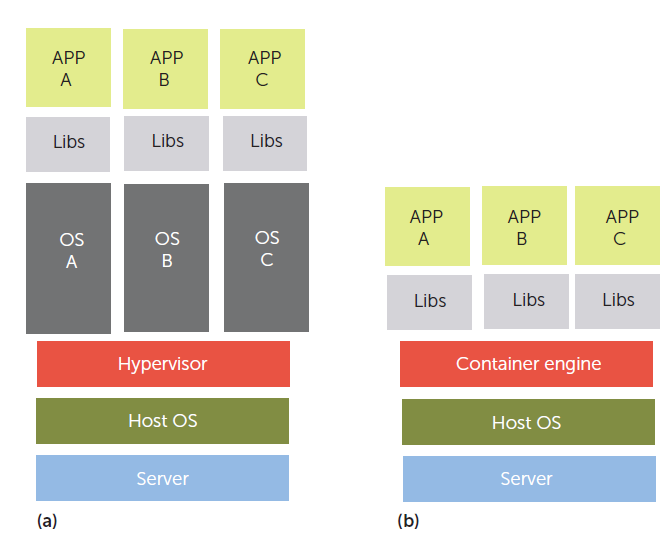
\includegraphics[width=0.7\linewidth]{resources/eea3da004befcc5437960cbc868be634.png}
    \caption{Architectural comparison of (a) virtual machine and (b) container \cite{bernsteinContainersCloudLXC2014}}
    \label{fig:vms-vs-containers}
\end{figure}

\section{Container Orchestration}

As the number of concurrently running containers grows, managing them quickly becomes challenging. Therefore, some form of automation is required to ease this orchestration process at scale. This is precisely the issue that container orchestration (CO) tools aim to solve. Similar to an orchestrator for an orchestra, CO technologies ensure that distributed containers work together harmoniously. By employing OC frameworks, enterprises and organisations can improve how resources are allocated, as well as simplify how they manage containers in cloud native settings \cite{truyenComprehensiveFeatureComparison2019}.

CO frameworks such as Kubernetes and Docker Swarm effectively manage the deployment, scaling, and networking of containers across multiple machines, allowing said machines to form clusters. These clusters are interconnected computers act as unified computing units that can handle containerised workloads, offloading the management responsibilities (connectivity, workload scheduling, scaling, resource allocation, etc.) from application developers \cite{Nodes, UsingMinikubeCreate}. In other words, from the developer's perspective, the cluster can be treated as a single computing unit to schedule workload. This configuration allows containerised applications to be distributed across multiple nodes in a straightforward manner. The design pattern is known as \textit{distributed application}, which is one of the most common design pattern in cloud computing due to its scalability and resiliency \cite{fehling2014cloud,kratzkeUnderstandingCloudnativeApplications2017}.

CO platforms compliment these benefits of distributed and containerised applications by minimising the management overhead, reducing the complexity of maintaining such configuration. The importance of workload distribution and containerisation in cloud infrastructure combine with the added benefits of CO platforms make them an important topic for research in both academia and industry. This focus on CO platforms and cloud-native application principles was revealed to be the research topic that gathered the most attention in a 2017 study \cite{kratzkeUnderstandingCloudnativeApplications2017}. The cloud space has evolved a lot since then. However, CO platforms still play a central role in today's cloud. The prevelant of CO platforms can be seen from the popularity of Kubernetes as a project, which will be discussed in section \ref{kubernetes}

\section{Cloud-native}
The Cloud-Native Computing Foundation (CNCF), part of the Linux Foundation, is an organisation that seeks to drive forward the cloud-native technologies and practices. They are the leading body in terms of setting best-practices recommendations in the cloud-native space. Many of the projects that they support, such as Kubernetes, Prometheus, HELM, and ArgoCD become de facto tools for cloud-native application development, monitoring, orchestration, and deployment. CNCF defined cloud-native as technologies that enable the development and deployment of scalable applications in cloud environments \cite{cloudnativecomputingfoundationWhoWeAre}. The application could be hosted on public, private, or hybrid cloud. However, in order to support the previously mentioned requirements, they usually possess the following attributes:

\begin{enumerate}
\item
  \textbf{Containers}: Compact, self-sufficient units containing all necessary components to run software, promoting uniformity from development through to deployment.
\item
  \textbf{Service Meshes}: Infrastructure layer that facilitates direct and manageable communication within microservices setups, enhancing clarity and control over service interactions.
\item
  \textbf{Microservices}: Design philosophy that organises applications into a network of small, independent services, each fulfilling a specific atomic function.
\item
  \textbf{Immutable Infrastructure}: Method that involves renewing or reconstructing infrastructure elements instead of modifying them, aiming to minimise discrepancies and prevent failures.
\item
  \textbf{Declarative APIs}: Interfaces that enable developers to define their requirements explicitly without detailing the execution process, streamlining application oversight by hiding the complexity of the underlying operations.
\end{enumerate}

\section{Kubernetes}\label{kubernetes}
\subsection{Background}

Developed by Google and later donated to the CNCF, Kubernetes is an open-source CO platform for automating the deployment, scaling, and operation of application containers \cite{Kubernetes}. Currently, it is one of the most popular cloud-native technologies with over 111,000 stars on GitHub, and has been accepted as the industry standard for container orchestration \cite{truyenComprehensiveFeatureComparison2019, KubernetesKubernetesProductionGrade}. It's specifically built to scale — capable of orchestrating thousands of containers across multiple environments (public, private and hybrid clouds).

Kubernetes offers several key features that make it well-suited for cloud-native application management:

\begin{itemize}

\item \textbf{Automated Scheduling}: Container placement in a cluster is done by automatically scheduling workloads considering resource availability and constraints to maximize infrastructure efficiency. 

\item \textbf{Self-Healing}: Kubernetes monitors the health of containers and nodes in the cluster and attempt to recover them in case of failures through initiating restart or rescheduling tasks.

\item \textbf{Horizontal Scaling}: Applications can adjust the number of container instances based on real-time demand automatically or manually in response to specified metric(s).

\item \textbf{Service discovery and load balancing}: Service discovery is simplified via the use of DNS names or IP addresses, with the network traffic being evenly distributed among container.

\item \textbf{Storage Orchestration}: Containers can have storage set up that is handled automatically with a wide variety of options including local storage, cloud-provisioned storage, and network file systems.

\item \textbf{Secret and Configuration Management}: Kubernetes handle sensitive data such as passwords, tokens, and configuration details and ensure that only the designated containers have access to them. 

\end{itemize}

In addition to its core functionality, Kubernetes has fostered a diverse portfolio of supportive tools and services such as Helm for package management, Prometheus for monitoring purposes, and ArgoCD for continuous delivery \cite{Helm, prometheusOverviewPrometheus, ArgoCDDeclarative}. This ecosystem plays a significant role in solidifying Kubernetes' central position in the modern cloud-native landscape.

\subsection{Distributions}
As a widely adopted tool across various industry, it is impossible for the upstream Kubernetes distribution to cater to all the different requirements and use-cases of its user. Thus, different Kubernetes \textit{distributions} emerged to address these specific needs, such as light-weight deployment and managed deployment \cite{bohmProfilingLightweightContainer2021, pereiraferreiraPerformanceEvaluationContainers2019}. From the licensing and management perspective, Kubernetes distributions largely falls into two categories: open-source (self-managed) and proprietary (managed).

\subsubsection{Open-source Kubernetes Distributions}

For organisations that prioritise flexibility, one potential option is to adopt an open-source Kubernetes distribution. Due to the lack of standards, there are certain differences between cloud service providers. According to Truyen et al. \cite{truyenManagingFeatureCompatibility2020}, these discrepancies largely fall into the following groups: cluster architecture and setup; framework customization interfaces; and feature incompatibilities. The disparity between vendors can create compatibility challenges when the need for platform migration arises. Open-source solutions' main strength is mitigating the risk of vendor lock-in, as well as minimising the operational cost. The differences will be discussed in further detail in the Related Works section.

\subsubsection{Managed Kubernetes Distributions}

Despite the high degree of customisability and flexibility that the open-source solutions offer, they lack the advanced features that managed Kubernetes distributions offer. As a result, there is a significant disparity in adoption, with organisations favouring managed solutions over open-source ones \cite{redhatinc.StateKubernetesSecurity2024}.


\section{The Cloud}

Cloud computing is a paradigm that enables companies to utilise computing resources over the internet without the need to manage infrastructure directly. According to the US National Institute of Standards and Technology, the cloud facilitates "ubiquitous, convenient, on-demand network access to a shared pool of configurable computing resources (e.g., networks, servers, storage, applications, and services) that can be rapidly provisioned and released with minimal management effort or service provider interaction" \cite{editorCloudComputingGlossary}. This offers businesses significant flexibility, scalability, and cost savings. Cloud services can be divided into three primary deployment models: Public Cloud, Private Cloud, and Hybrid Cloud \cite{jadejaCloudComputingConcepts2012}.

\subsection{Public Cloud}

The public cloud is the most commonly adopted deployment model. Naturally, all leading cloud providers such as Amazon, Microsoft, and Google offer their variant of public cloud. In this model, organisations can rent necessary resources based on their usage from a shared pool. This allows organisations to utilise cloud resources without investing in physical infrastructure upfront. Furthermore, public cloud also offers tenants the ability to elastically adjust resource levels according to demand, scaling up or down as needed to potentially reduce costs \cite{suleiman2012understanding}. However, public clouds are traditionally considered less secure than other cloud models due to being hosted by third-party vendors \cite{jadejaCloudComputingConcepts2012}. 

In the context of managed Kubernetes, some major public cloud options are Amazon Elastic Kubernetes Service (EKS), Google Kubernetes Engine (GKE), Azure Kubernetes Service (AKS), Red Hat OpenShift \footnote{At the time of writing, OpenShift offer 4 public cloud provider options for cloud-hosted infrastructure: AWS, Azure, Google, and IBM \cite{OpenShiftContainerPlatform}}, and VMware Tanzu \cite{AmazonEKSCustomers, maEurekaHumanLevelReward2023, nickomangAzureKubernetesService, redhatinc.RedHatOpenShift, VMwareTanzuPlatform}.

This thesis focuses strictly on public cloud managed Kubernetes offerings, due to the limited availability of pricing information for the self-managed/private cloud option \cite{redhatinc.RedHatOpenShift}.

\subsection{Private Cloud}

In a private cloud setup, organisations obtain dedicated cloud environments exclusively for their usage. In contrast with the public cloud, a private cloud ensures isolation of infrastructure and services, offering enhanced control, customisation, and security. Private clouds are often hosted on-premise. This dedicated environment can be tailored to meet the specific needs of the organisation \cite{jadejaCloudComputingConcepts2012}.

\subsection{Hybrid Cloud}

A hybrid cloud deployment allows users to access features from both private and public clouds, taking advantage of both environments \cite{jadejaCloudComputingConcepts2012, dash2016governance}. This model allows organisations to run sensitive or critical workloads in-house, while leveraging the public cloud for less sensitive tasks. In addition, the integration of public cloud into the deployment also accommodates scaling requirements during peak demand, thus letting organisations optimise for both security and cost-efficiency \cite{huangAchievingBigData2014}.




\section{Interest in Kubernetes and Managed Kubernetes}

\subsection{Google Trends}

\FloatBarrier  

\begin{figure}
    \centering
    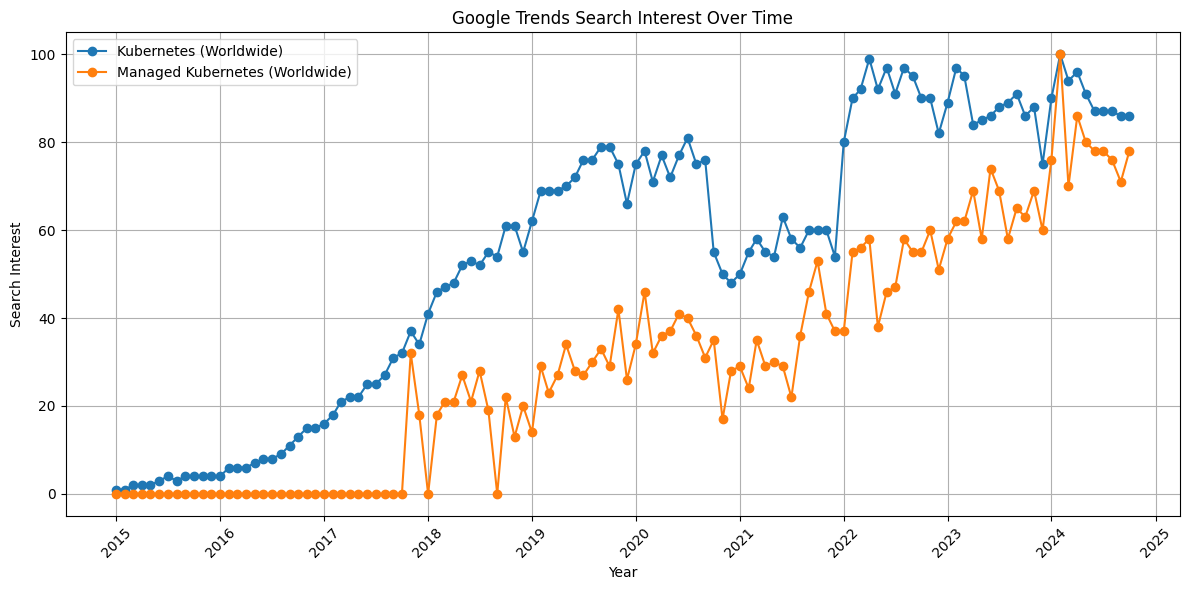
\includegraphics[width=1\linewidth]{resources/d2a89eeeda76d50039bc6f5d3a97c41b.png}
    \caption{Google Trends search interest in Kubernetes vs managed Kubernetes}
    \label{fig:search-interests-kubernetes-vs-managed-kubernetes}
\end{figure}

To provide context for the topic covered in this thesis, this section looks at the popularity of Kubernetes and managed Kubernetes by examining Google Trends search data and the yearly publications data from the Web of Science database. Although Google Trends is not considered a reliable research tool, Kratzke et al. proposed that it can serve as a resource for spotting “industrial buzzwords” and new trends in the technology sector \cite{kratzkeUnderstandingCloudnativeApplications2017}. By combining this data with an analysis of research publications, we can gain insights into evolving trends in both the industry and in academia. The keywords examined are “Kubernetes” and “managed Kubernetes” (case-insensitive) and the timeframe spans from the earliest data-point to October 2024, which is one month prior to the completion of this thesis.

The graph depicted in Figure \ref{fig:search-interests-kubernetes-vs-managed-kubernetes} shows the search interest on Google for “Kubernetes” compared to “managed Kubernetes”. From the plot, it can be discerned that there is a steady rise in popularity for Kubernetes since its introduction until the peak around 2022, after which the search interest stabilises.

One noteworthy aspect is the drop in search activity observed in 2021; however, the reason behind this decline remains ambiguous. Similar search trends were observed for various cloud-native technologies such as Docker and Fluentd, showing comparable decreases. This commonality suggests that although the root cause remains unknown, this change may have influenced a wide array of adjacent technologies in the cloud-native sphere.

The Google Trends data also highlights a convergence in interest for Kubernetes and managed Kubernetes, especially in recent years. The growing preference for managed Kubernetes could indicate a rising awareness among users and businesses about the benefits of managed solutions.

The preference for managed Kubernetes is further supported through industrial reports and surveys. For instance, a 2022 report by Canonical indicated that only 19.3\% of respondents use native (self-managed) Kubernetes \cite{canonicalKubernetesCloudNative2022}. Similarly, Red Hat's 2024 state of Kubernetes security report showed comparable data, with just 23\% of respondents using self-managed Kubernetes \cite{redhatinc.StateKubernetesSecurity2024}.

\subsection{Research Publications}

\FloatBarrier

\begin{figure}
    \centering
    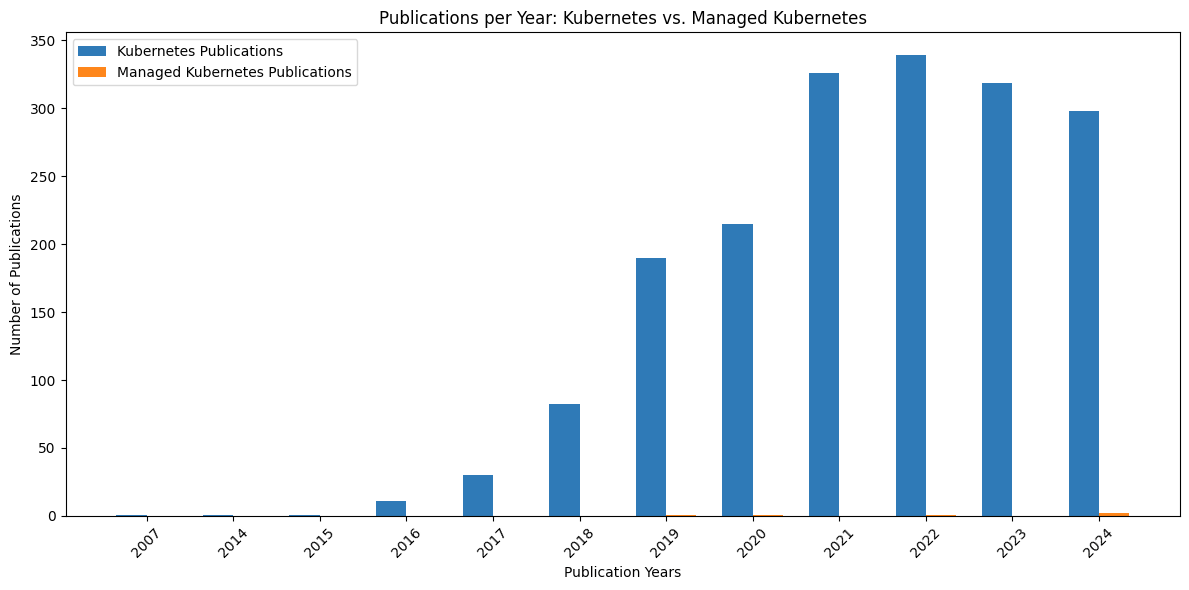
\includegraphics[width=1\linewidth]{resources/55ccf3419c03248ff5a2383d4ae63366.png}
    \caption{Annual Research Publications on Kubernetes and managed Kubernetes}
    \label{fig:research-publications-kubernetes-and-managed-kubernetes}
\end{figure}


This process of analysing academic interest for the given topics involved collecting information on the yearly publication count through the Web of Science result analysis tool. This annual publication data, shown in Figure \ref{fig:research-publications-kubernetes-and-managed-kubernetes}, reflects a steady increase in Kubernetes-related publications until the peak in 2022. This trends aligns with the results demonstrated by the Google Trends data.

Nevertheless, it is worth noting that managed Kubernetes has not received the same level of attention in academic research as it has in Google Trends. There was only a rather limited number of publications annually from 2019 to 2024, with only one or two publications per year. This disparity indicates that there could be potential for further academic investigation into managed Kubernetes (e.g. features, performance, and costs), similar to Ferreira’s study \cite{pereiraferreiraPerformanceEvaluationContainers2019}.

Regarding the observed peak, a 2019 study by Truyen et al. \cite{truyenComprehensiveFeatureComparison2019} proposed that container orchestration technologies were entering the peak of the Gartner hype cycle. However, both the Google Trends data and the number of annually published articles seem to suggest otherwise. From these insights, it appears that Kubernetes likely reached its peak in popularity around 2022.

These statistics indicate a rising interest in both Kubernetes and managed Kubernetes, highlighting the relevance of the thesis topic. The increasing interest in managed Kubernetes, combined with the lack of research evaluating managed Kubernetes solutions, demonstrated a potential for further academic exploration and analysis to address this gap.

\section{Related Works}
\subsubsection{Differences Between K8s vendors and vendor lock-in}
The paper "Managing Feature Compatibility in Kubernetes: Vendor Comparison and Analysis" by Truyen et al \cite{truyenManagingFeatureCompatibility2020}. look at three major Kubernetes distributions (EKS, AKS, GKE) and compare them in terms of feature compatibility and potential of vendor lock-in. The main groups of differences proposed are:

\begin{itemize}

\item \textbf{Architectural}: Differences in terms of the way the platform is implemented. For example, scheduler, controlplane, pod node limitations, etc. 
\item \textbf{Customization interfaces}: Differences in terms of how Kubernetes components can be configure. For example, Service accounts, CNI choices, volume management, etc.
\item \textbf{Feature incompatibilities}: Differences in terms of feature availability. For example, API resources, Custom Resource Definitions (CRDs), etc.

\end{itemize}

These divergences can bring migration challenges, which introduces a risk called \textit{vendor lock-in}. Vendor lock-in happens when an organisation becomes dependent on a product, while alternative options require significant efforts (e.g. costs, technical, legal) \cite{opara2016critical}. Further details of the differences are covered below.


\subsubsection{Architectural Differences}

It was identified that there are fundamental differences in terms of architecture between the examined distributions. A list of the differences can be seen from Table \ref{tab:architecture-diff-k8s-distro}. Red Hat OpenShift Container Platform (OCP) was not covered in the paper, and it is not the focus of this thesis to identify architectural differences between these distributions. However, to gain a broad idea of their differences, we can identify that one key difference is the OS requirements. Acording the paper, all three distributions examined (AKS, EKS, and GKE) have support for Windows Server nodes \cite{truyenManagingFeatureCompatibility2020}. This, however, is not the case for Red Hat OpenShift Container Platform (OCP). At the time of writing, Red Hat CoreOS (RHCOS) is the "the only supported operating system for OpenShift Container Platform control plane, or master, machines" \cite{RedHatEnterprise}.

Furthermore, for OCP 4.1 the Maximum nodes per cluster for OCP is 2,000 \cite{Chapter6Planning}. OCP 4.1 was released in June 2019, which should make the available specifications comparable to those of AKS, EKS, and GKE in the paper from Truyen et al \cite{truyenManagingFeatureCompatibility2020}. As of the time of writing, the maximum nodes limit has not increased with the latest version of OCP \cite{Chapter4Planning}.


\begin{table}
    \centering
    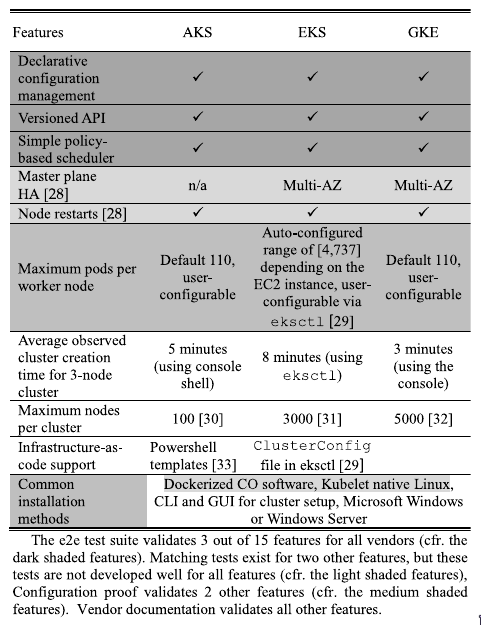
\includegraphics[width=0.6\linewidth]{resources/Pasted image 20241123075148.png}
    \caption{Architectural differences between three major Kubernetes distribution \cite{truyenManagingFeatureCompatibility2020}}
    \label{tab:architecture-diff-k8s-distro}
\end{table}

\FloatBarrier



\subsubsection{Customization Interfaces}



Framework customisation interfaces are the means exposed to customers to customise their Kubernetes environment \cite{truyenManagingFeatureCompatibility2020}. An example of framework customisation difference between the distributions is the default container network interface (CNI) used for a standard cluster. The CNI for AKS, EKS, and GKE can be seen in Table \ref{tab:kube-distro-cni-diff}. From this table, kubenet appears to be a common choice for CNI among the managed Kubernetes distribution examined by Truyen et al \cite{truyenManagingFeatureCompatibility2020}. OCP, on the other hand, uses OVN-Kubernetes as the default CNI for its cluster \cite{Chapter23OVNKubernetes}.


\begin{table}
    \centering
    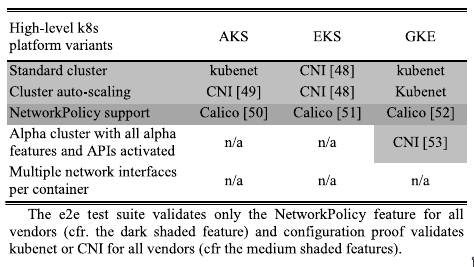
\includegraphics[width=0.6\linewidth]{resources/Pasted image 20241123082858.png}
    \caption{CNI Differences between AKS, EKS, and GKE \cite{truyenManagingFeatureCompatibility2020}}
    \label{tab:kube-distro-cni-diff}
\end{table}

\FloatBarrier

\subsubsection{Feature Incompatibilities}


The final group of potential differences between Kubernetes distributions is feature incompatibilities between them. These differences manifest itself as disparities in the available API and custom resource definitions (CRDs). In practice, this determines what functionalities is available to use within the cluster. For instance, although Security Context is a universal concept that exists in Kubernetes and all the downstream Kubernetes distributions, Security Context Constraint (SCC) only exists in OCP \cite{ConfigureSecurityContext, ManagingSecurityContext}. These discrepancies, as identified by Truyen et al. \cite{truyenManagingFeatureCompatibility2020}, could potentially lead to difficulties in platform migration. In the case of OCP SCCs, applications from another vendor that does not have sufficient SCC privileges configured might not run successfully on OCP \cite{ConfigureSecurityContext}.

\subsubsection{Ease of Migration Analysis}

Due to the mentioned differences between platforms, migrating from one platform to another can prove to be a challenging procedure. Truyen et al. \cite{cloudnativecomputingfoundationFrequentlyAskedQuestions2018} evaluated AKS, EKS, and GKE in terms of pair-wise migratability mapping across these differences. 

The paper discussed potential errors in the recorded findings due to some test results (coloured in a brown-shade) being inconsistent with the official documentation. After adjusting for these errors, EKS possesses the lowest number of incompatible occurrences, making it the most configurable distribution out of the ones examined. In other words, when strictly considering their compatibility with native Kubernetes' customisation interfaces, EKS is more compatible than the other two vendors \textit{after potential configurations}.

GKE, on the other hand, has the highest number of Kubernetes features that work \textit{out-of-the-box}. This means that out-of-the-box with zero configuration, GKE is the most compatible with native Kubernetes' feature set, making it the more feature-rich distribution.

In short, EKS is more compatible when taking into account potential configuration steps, while GKE is more compatible while taking into account the out-of-the-box state of the distribution.

The work shown that there are non-negligible differences even among major players in the managed Kubernetes space and the compatibility between evaluated platforms. However, the paper did not assess the importance of the features provided by the platforms as well as the differences in cost of operation. In addition, OCP was not evaluated in the study. As one of the most popular managed Kubernetes distributions, there are potential valuable insights to be gained from examining OCP and comparing it against other offerings \cite{redhatinc.StateKubernetesSecurity2024, vrabicDigitalTwinsUnderstanding2018, portworxKubernetesAdoptionSurvey2021, broadcomStateKubernetes20232023}.

\chapter{Methodology}


\chapter{Results and Discussion}


\chapter{Conclusion}

- Concluding remarks and potential aspects to look at future works.


















%%  LIITTEET  ------------------------------------------

% \appendix
% \chapter{Ut purus elit}

% Lorem ipsum dolor sit amet, consectetuer adipiscing elit. Ut purus
% elit, vestibulum ut, placerat ac, adipiscing vitae, felis. Curabitur
% dictum gravida mauris. Nam arcu libero, nonummy eget, consectetuer id,
% vulputate a, magna. Donec vehicula augue eu neque. Pellentesque
% habitant morbi tristique senectus et netus et malesuada fames ac
% turpis egestas. Mauris ut leo. Cras viverra metus rhoncus sem. Nulla
% et lectus vestibulum urna fringilla ultrices. Phasellus eu tellus sit
% amet tortor gravida placerat. Integer sapien est, iaculis in, pretium
% quis, viverra ac, nunc. Praesent eget sem vel leo ultrices
% bibendum. Aenean faucibus. Morbi dolor nulla, malesuada eu, pulvinar
% at, mollis ac, nulla. Curabitur auctor semper nulla.  Donec varius
% orci eget risus. Duis nibh mi, congue eu, accumsan eleifend, sagittis
% quis, diam. Duis eget orci sit amet orci dignissim rutrum.

% Nam dui ligula, fringilla a, euismod sodales, sollicitudin vel,
% wisi. Morbi auctor lorem non justo. Nam lacus libero, pretium at,
% lobortis vitae, ultricies et, tellus. Donec aliquet, tortor sed
% accumsan bibendum, erat ligula aliquet magna, vitae ornare odio metus
% a mi. Morbi ac orci et nisl hendrerit mollis. Suspendisse ut
% massa. Cras nec ante. Pellentesque a nulla.  Cum sociis natoque
% penatibus et magnis dis parturient montes, nascetur ridiculus
% mus. Aliquam tincidunt urna. Nulla ullamcorper vestibulum
% turpis. Pellentesque cursus luctus mauris.

% \section{Fusce mauris}

% Fusce mauris. Vestibulum luctus nibh at lectus. Sed bibendum, nulla a
% faucibus semper, leo velit ultricies tellus, ac venenatis arcu wisi
% vel nisl.  Vestibulum diam. Aliquam pellentesque, augue quis sagittis
% posuere, turpis lacus congue quam, in hendrerit risus eros eget
% felis. Maecenas eget erat in sapien mattis porttitor. Vestibulum
% porttitor. Nulla facilisi.  Sed a turpis eu lacus commodo
% facilisis. Morbi fringilla, wisi in dignissim interdum, justo lectus
% sagittis dui, et vehicula libero dui cursus dui. Mauris tempor ligula
% sed lacus. Duis cursus enim ut augue. Cras ac magna.  Cras
% nulla. Nulla egestas. Curabitur a leo. Quisque egestas wisi eget
% nunc. Nam feugiat lacus vel est. Curabitur consectetuer.

\renewcommand{\bibname}{References (IEEE)}
\printbibliography
% \bibliography{references.bib}

\end{document}
